\section{Results}\label{sec:results}
\mr{TODO: The mean density and cross power spectrum $\chi^{2}$ diagnostics do not reveal any signature of remaining systematic effects -- given all the available templates. But we could be missing some unknown maps. There are some calibration maps made by Aaron which I need to look into. I did not use the Gaia stellar map for training-- Zhou et al has a discussion on why it should not be used. But I plan to apply some cuts based on imaging (e.g., poor depth, high stellar density and extinction) to see if those impact the best fit estimates. Next, I will study how changing the lowest ell used could affect our results. }

\subsection{Lognormal Mocks}

Corner plots of the PNG parameter $\fnl$ and bias coefficient are shown in Fig. \ref{fig:mcmc_mocks} for fitting the mean power spectrum of the mocks, with and without $\fnl$. Maximum-A-Posteriori estimates and marginalized mean, median and $1\sigma$ quantiles are summarized in Tab. \ref{tab:mocksmcmc}. Comparing DECaLS North with sky coverage $0.14$ to full DESI with $0.40$, we find the constraint improve by a factor of $1.9$ which is slightly more than $\sim f_{\rm SKY}^{-1/2}$, 1.7. while As a robustness test, we also fit the mean power spectrum of the $\fnl=100$ mocks using the covariance matrix estimated from the $\fnl=0$ mocks. We find that the constraints improve by a factor of $4.2$, due to a higher signal to noise ratio.

\begin{table*}
  %\begin{center}
    \caption{Maximum-A-Posteriori (MAP) and marginalized mean estimates for $\fnl$ from fitting the mean power spectrum of the mocks. Degree of freedom is 34 (37 data points - 3 parameters).}   
    \label{tab:mocksmcmc}  
   \centerline{%
    \begin{tabular}{clllllll}
    \hline
    \hline
   &  & 	  & & & $\fnl$ &  \\
   \cmidrule(r{.7cm}){4-7}    
True $\fnl$ &  Footprint   &  Observable & 	Best fit  & Mean & $ 68\%$ CL & $ 95\%$ CL & $\chi^{2}$ \\
    \hline
$76.92$ & DESI & log$C_{\ell}$           & $ 77.67$& $ 77.67$& $ 77.17<\fnl< 78.16$& $ 76.71<\fnl< 78.64$ &   38.8\\
$76.92$ & DESI & $C_{\ell}$              & $ 77.67$& $ 77.65$& $ 77.17<\fnl< 78.14$& $ 76.70<\fnl< 78.60$ &   39.0\\
$76.92$ & DESI & log$C_{\ell}$ + $f_{\rm NL}=0$ cov & $ 77.70$& $ 77.71$& $ 77.25<\fnl< 78.17$& $ 76.81<\fnl< 78.63$ &   39.9\\
$76.92$ & DESI & $C_{\ell}$ + $f_{\rm NL}=0$ cov & $ 77.03$& $ 77.02$& $ 76.93<\fnl< 77.12$& $ 76.83<\fnl< 77.22$ &  207.6\\
\hline
$0$ & DESI         &  log$C_{\ell}$     & $  0.36$& $  0.36$& $  0.06<\fnl<  0.65$& $ -0.23<\fnl<  0.94$ &   35.7\\
$0$ & DECaLS North &  log$C_{\ell}$     & $  0.07$& $  0.06$& $ -0.47<\fnl<  0.60$& $ -1.00<\fnl<  1.12$ &   26.7\\
$0$ & DECaLS South &  log$C_{\ell}$     & $  0.67$& $  0.67$& $  0.13<\fnl<  1.22$& $ -0.40<\fnl<  1.75$ &   34.3\\
$0$ & BASS+MzLS    &  log$C_{\ell}$     & $  0.83$& $  0.82$& $  0.25<\fnl<  1.40$& $ -0.31<\fnl<  1.96$ &   39.4\\
\hline
    \end{tabular}
    }
\end{table*}


\begin{figure*}
    \centering
    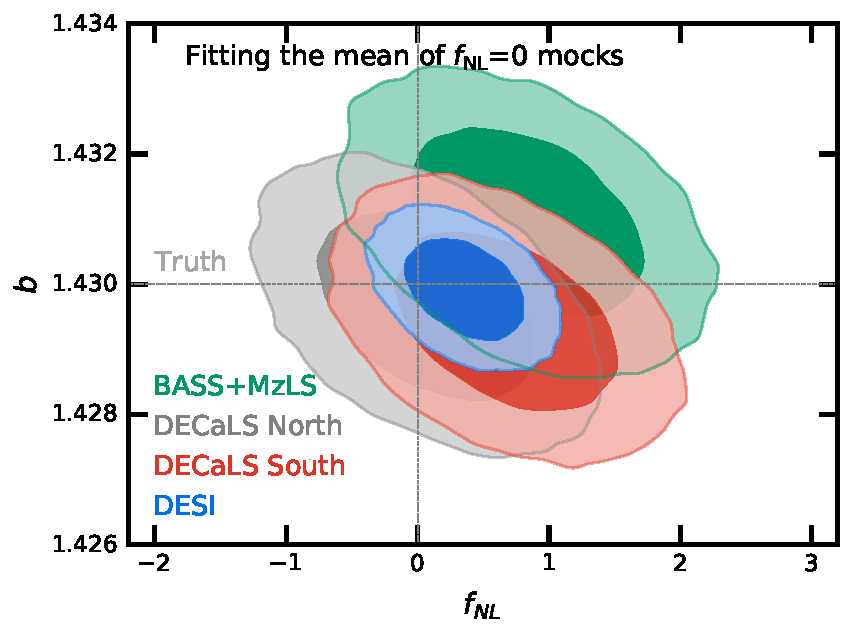
\includegraphics[width=0.45\textwidth]{figures/mcmc_zero.pdf} 
    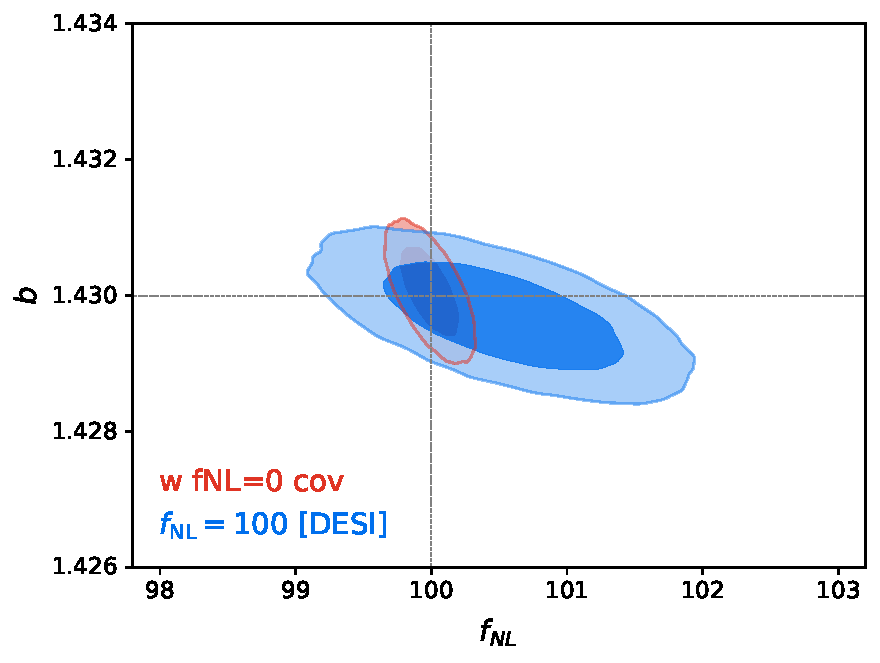
\includegraphics[width=0.45\textwidth]{figures/mcmc_po100.pdf} 
    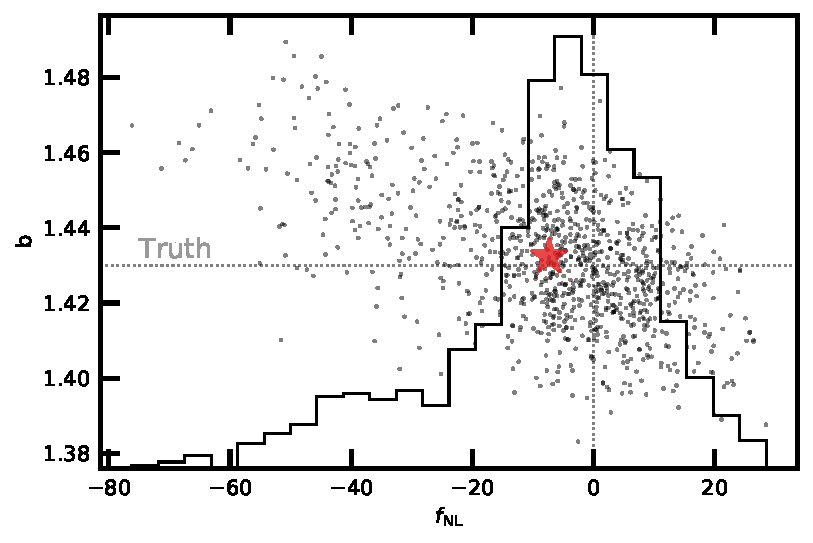
\includegraphics[width=0.45\textwidth]{figures/bestfit_zero.pdf} 
    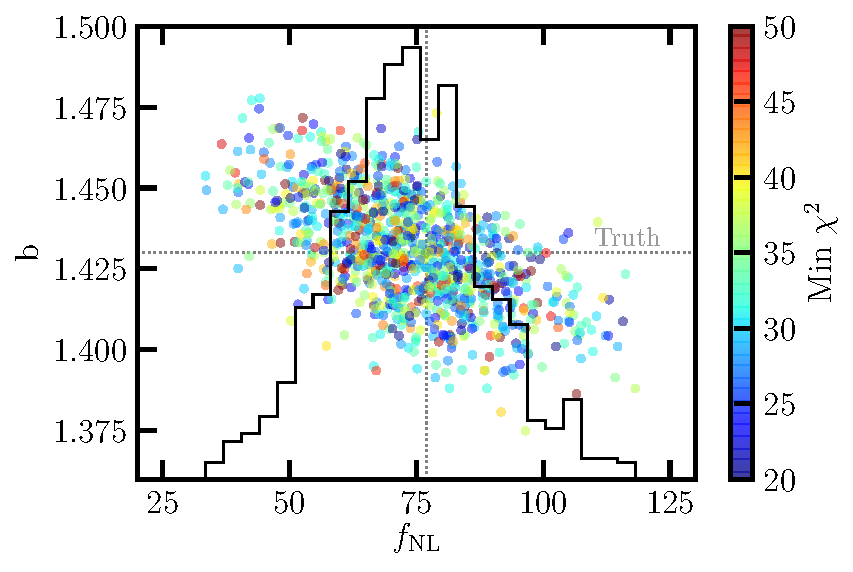
\includegraphics[width=0.45\textwidth]{figures/bestfit_po100.pdf}         
    \caption{Top: 68\% and 95\% confidence contours for $\fnl=0$ (left) and $100$ (right) mocks. Using the $\log C_{\ell}$ fitting yield constraints that are insensitive to the covariance used. Bottom: best fit estimates from fitting 1000 lognormal mocks with $\fnl=0$ (left) and $100$ (right) in the DESI footprint. The truth values are represented by vertical and horizontal lines.}\label{fig:mcmc_mocks}
\end{figure*}



\subsection{DR9 LRGs}




\begin{table*}
    \caption{Maximum-A-Posteriori (MAP) and marginalized mean estimates for $\fnl$ from fitting power spectrum of DR9 LRGs before and after correcting for systematics. Degree of freedom is 34 (37 data points - 3 parameters).}
    \label{tab:dr9method}
   \centerline{%     
    \begin{tabular}{llllllll}
    \hline
    \hline
   &  & 	  & & $\fnl$ &  &  \\
   \cmidrule(r{.7cm}){3-6}
Footprint   & Method & 	Best fit  & Mean & $ 68\%$ CL & $ 95\%$ CL & $\chi^{2}$ \\
    \hline
DESI                      & No Weight   & $113.18$& $115.49$& $ 98.14<\fnl<132.89$& $ 83.51<\fnl<151.59$ &   44.4\\
DESI                      & Linear (All Maps)& $ 36.05$& $ 37.72$& $ 26.13<\fnl< 49.21$& $ 16.31<\fnl< 62.31$ &   41.1\\
DESI                      & Linear (Conservative I)& $ 49.58$& $ 51.30$& $ 38.21<\fnl< 64.33$& $ 27.41<\fnl< 78.91$ &   38.8\\
DESI                      & Linear (Conservative II)& $ 36.63$& $ 38.11$& $ 26.32<\fnl< 49.86$& $ 16.36<\fnl< 63.12$ &   39.6\\
DESI                      & Nonlinear (Cons. II)& $ 28.58$& $ 29.79$& $ 18.91<\fnl< 40.59$& $  9.47<\fnl< 52.73$ &   34.6\\
DESI                      & Nonlin. (Cons. II+nStar)& $ 16.63$& $ 17.52$& $  7.51<\fnl< 27.53$& $ -1.59<\fnl< 38.49$ &   35.2\\
DESI                      & Nonlin. (All Maps+nStar)& $ -5.87$& $ -9.19$& $-21.45<\fnl<  2.40$& $-33.81<\fnl< 12.06$ &   39.5\\
DESI (imag. cut)          & Nonlin. (Cons. II)& $ 29.16$& $ 30.57$& $ 19.05<\fnl< 42.18$& $  9.01<\fnl< 54.81$ &   35.8\\
DESI (comp. cut)          & Nonlin. (Cons. II)& $ 28.07$& $ 29.48$& $ 18.38<\fnl< 40.50$& $  8.81<\fnl< 53.10$ &   34.5\\
DESI                      & Nonlin. (Cons. II)+$f_{\rm NL}=76.92$ Cov& $ 31.62$& $ 33.11$& $ 20.94<\fnl< 45.24$& $ 10.56<\fnl< 59.16$ &   33.5\\
\hline
BASS+MzLS                 & Nonlin. (Cons. II)& $ 15.43$& $ 19.01$& $ -1.17<\fnl< 39.43$& $-19.19<\fnl< 63.56$ &   35.6\\
BASS+MzLS                 & Nonlin. (Cons. II+nStar)& $ 13.12$& $ 15.39$& $ -4.59<\fnl< 35.56$& $-24.88<\fnl< 59.31$ &   34.7\\
BASS+MzLS                 & Nonlin. (All Maps+nStar)& $ -3.73$& $ -6.34$& $-27.11<\fnl< 13.75$& $-47.44<\fnl< 33.94$ &   36.8\\
BASS+MzLS (imag. cut)     & Nonlin. (Cons. II)& $ 25.03$& $ 29.12$& $  6.16<\fnl< 52.44$& $-14.22<\fnl< 80.54$ &   36.2\\
BASS+MzLS (comp. cut)     & Nonlin. (Cons. II)& $ 16.99$& $ 20.90$& $  0.26<\fnl< 41.76$& $-18.30<\fnl< 67.12$ &   35.8\\
DECaLS North              & Nonlin. (Cons. II)& $ 41.02$& $ 44.89$& $ 23.33<\fnl< 66.78$& $  4.96<\fnl< 93.02$ &   41.1\\
DECaLS North              & Nonlin. (Cons. II+CALIBZ+HI)& $ 55.46$& $ 60.44$& $ 36.78<\fnl< 84.05$& $ 17.86<\fnl<112.81$ &   38.4\\
DECaLS North              & Nonlin. (Cons. II+nStar)& $ 31.45$& $ 34.78$& $ 14.14<\fnl< 55.79$& $ -5.81<\fnl< 80.80$ &   41.2\\
DECaLS North              & Nonlin. (All Maps+nStar)& $  0.81$& $ -5.68$& $-29.73<\fnl< 16.71$& $-53.15<\fnl< 36.19$ &   45.1\\
DECaLS North + islands & Nonlin. (Cons. II)& $ 41.05$& $ 44.82$& $ 23.58<\fnl< 66.08$& $  6.40<\fnl< 91.42$ &   40.7\\
DECaLS North (imag. cut)  & Nonlin. (Cons. II)& $ 43.27$& $ 48.39$& $ 24.60<\fnl< 72.50$& $  4.71<\fnl<101.42$ &   35.1\\
DECaLS North (comp. cut)  & Nonlin. (Cons. II)& $ 40.55$& $ 44.63$& $ 22.41<\fnl< 67.11$& $  3.95<\fnl< 94.06$ &   41.4\\
DECaLS South              & Nonlin. (Cons. II)& $ 31.24$& $ 33.21$& $ 14.89<\fnl< 52.40$& $ -5.11<\fnl< 74.35$ &   30.2\\
DECaLS South              & Nonlin. (Cons. II+CALIBZ+HI)& $ 33.79$& $ 37.50$& $ 17.71<\fnl< 57.42$& $ -0.31<\fnl< 80.94$ &   30.8\\
DECaLS South              & Nonlin. (Cons. II+nStar)& $ 14.34$& $  6.28$& $-21.19<\fnl< 30.01$& $-53.63<\fnl< 49.51$ &   31.9\\
DECaLS South              & Nonlin. (All Maps+nStar)& $-36.76$& $-32.01$& $-49.38<\fnl<-13.61$& $-65.26<\fnl<  7.52$ &   31.5\\
DECaLS South + DEC < $-30$ & Nonlin. (Cons. II)& $ 43.79$& $ 46.79$& $ 30.16<\fnl< 63.41$& $ 16.38<\fnl< 82.72$ &   23.8\\
DECaLS South (imag. cut)  & Nonlin. (Cons. II)& $ 26.47$& $ 23.36$& $  3.18<\fnl< 47.84$& $-57.69<\fnl< 71.39$ &   30.0\\
DECaLS South (comp. cut)  & Nonlin. (Cons. II)& $ 29.62$& $ 31.76$& $ 13.00<\fnl< 51.58$& $ -9.78<\fnl< 74.28$ &   29.7\\
   \hline
    \end{tabular}
}
\end{table*}


\begin{figure}
    \centering
    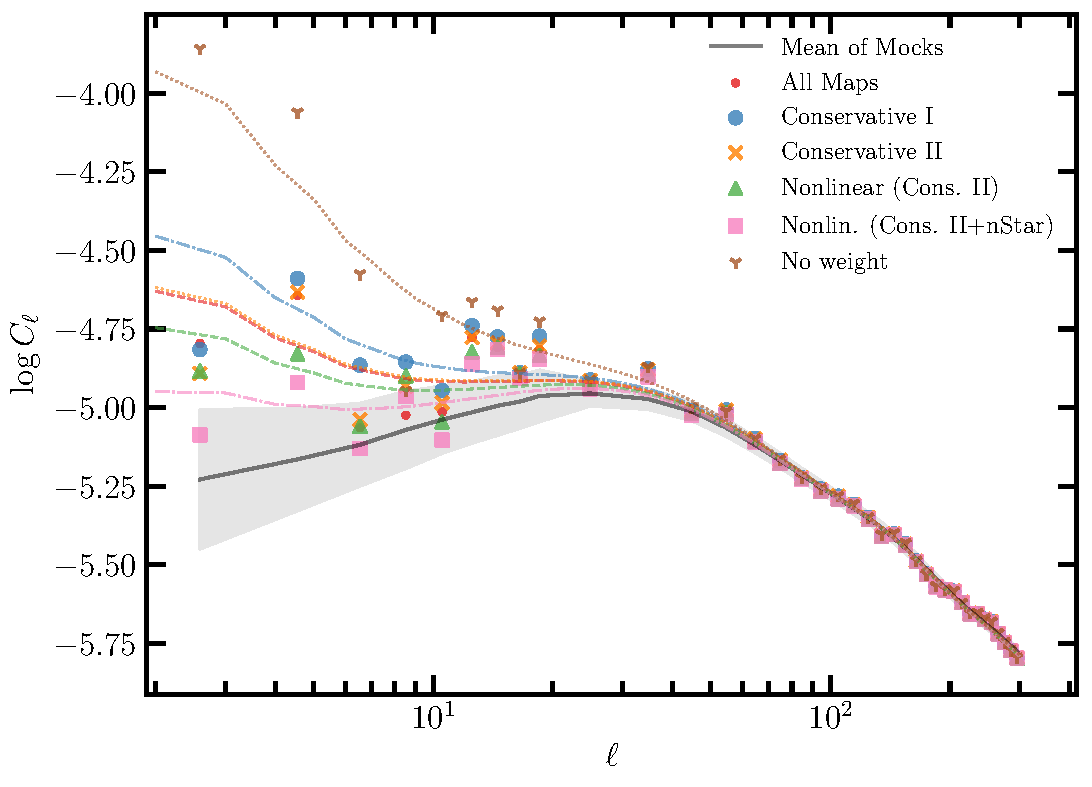
\includegraphics[width=0.45\textwidth]{figures/model_dr9.pdf} 
    \caption{Measured power spectrum of the DR9 LRG sample before and after correcting for systematics with their corresponding best fit theory predictions. The shade represents $1\sigma$ error constructed from the $\fnl=0$ mocks.}
    \label{fig:cl_dr9}
\end{figure}

\begin{figure}
\centering
    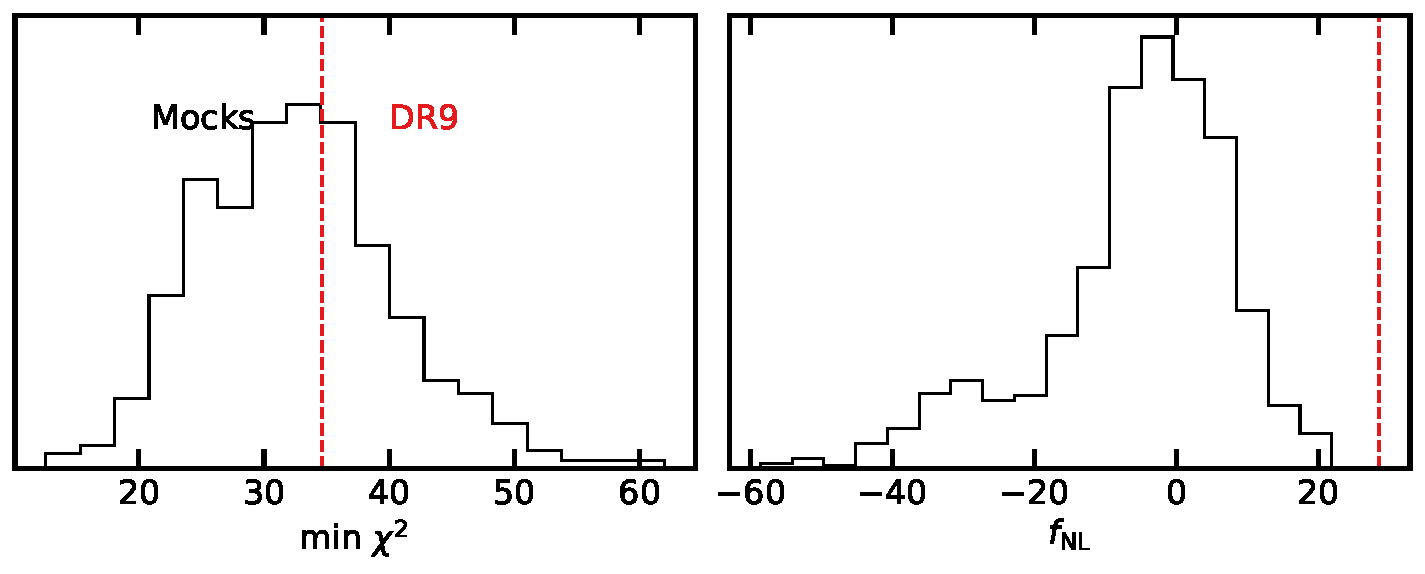
\includegraphics[width=0.45\textwidth]{figures/pdf_dr9vsmocks.pdf} 
    \caption{Best fit $\chi^{2}$ and $\fnl$ from fitting mocks (histograms) and DR9 (vertical line).}\label{fig:dr9vsmocks}
\end{figure}

\begin{figure}
    \centering
    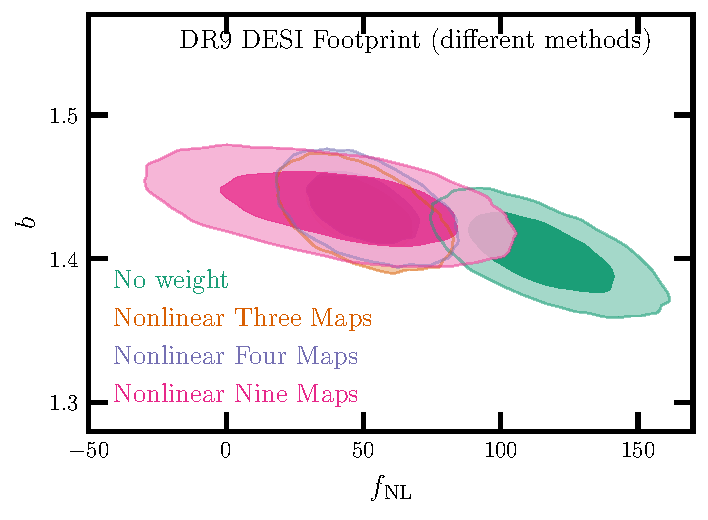
\includegraphics[width=0.45\textwidth]{figures/mcmc_dr9methods.pdf} 
    \caption{DR9 constraints. DESI footprint before and after applying various cleaning methods.}\label{fig:mcmc_dr9}
\end{figure}

\begin{figure}
    \centering
    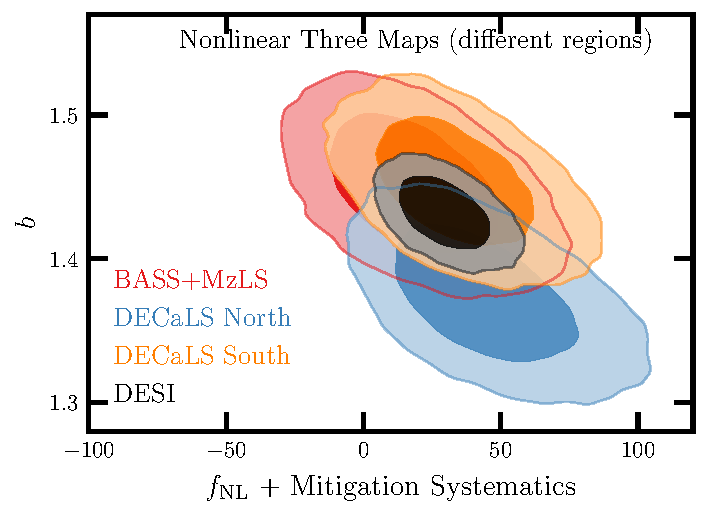
\includegraphics[width=0.45\textwidth]{figures/mcmc_dr9regions.pdf} 
    \caption{DR9 constraints. Each individual imaging survey versus the whole DESI footprint.}\label{fig:mcmc_dr9reg}
\end{figure}

\begin{figure*}
    \centering
    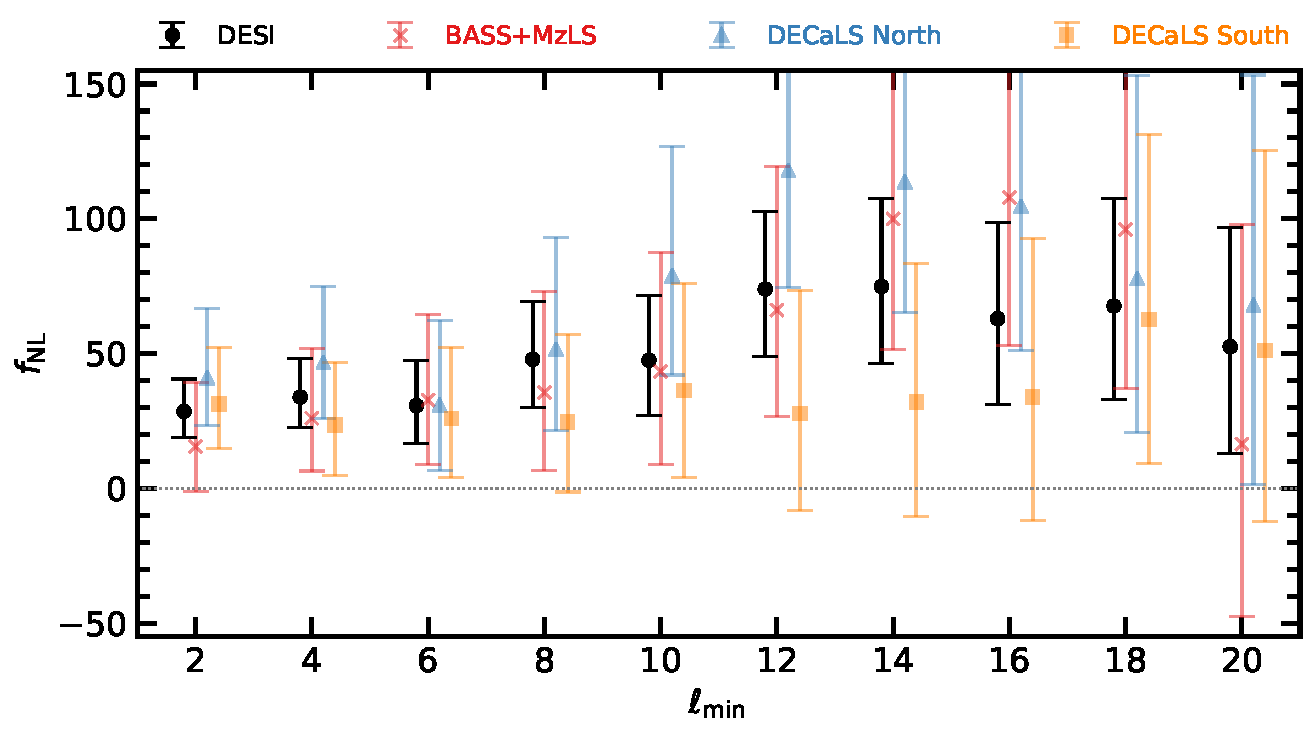
\includegraphics[width=0.95\textwidth]{figures/fnl_elmin.pdf}     
    \caption{DR9 Constraints. Mean estimates of $\fnl$ and its $65$\% and $95$\% errorbars after changing the lowest $\ell$ mode used in fitting.}\label{fig:mcmc_dr9elmin}
\end{figure*}
